\chapter{SDN Control Plane Scalability} \label{sec:sdn_scalability} 
\ifpdf
    \graphicspath{{Chapter1/Chapter1Figs/PNG/}{Chapter1/Chapter1Figs/PDF/}{Chapter1/Chapter1Figs/}}
\else
    \graphicspath{{Chapter1/Chapter1Figs/EPS/}{Chapter1/Chapter1Figs/}}
\fi

In this thesis we develop mechanisms to scale computer network functionality, by
redesigning the control plane.  In our exploration we employ extensively  he SDN
design paradigm and the \of protocol abstraction.  We chose the SDN design
approach due to two core functional properties.  On one hand, the clean
separation of the control and the forwarding plane in a network is inherently
backwards compatibility with existing network applications and interoperable
with existing network devices.  The evolution of the control plane of a network
doesn't affect forwarding plane protocol support, while SDN supports progressive
deployment in production networks without any forwarding performance penalty.
Secondly, the \of control abstraction is sufficiently generic to support a
diverse set of control approaches. The protocol supports reactive and proactive
control schemes, while the flow definition granularity is dynamically controlled
to match the application requirements. In the following chapters of this thesis
we employ the \of protocol to address two diverse network scalability problems. 

In this chapter we present an extensive performance analysis of the control
scalability of available SDN technologies. Our exploration aims to provide an 
in-depth presentation of the limitations of existing implementation efforts and
understand their impact in forwarding plane performance, as well as, provide a
set of tools which enable SDN developers to study the performance of their
network designs. The work focuses on implementations of version 1.0 of the \of
protocol, the only production-level protocol instantiation of the SDN paradigm.
We conduct our analysis using two measurement platforms: \oflops and \sdnsim.
\oflops is a high precision \of switch micro-benchmark platform. Using \oflops,
we implement a set of benchmark tests to characterise the performance of elementary
\of protocol interactions. \sdnsim is a macro-benchmark \of platform, which
extends the Mirage framework~\cite{madhavapeddy2013} to support large scale
\of-based network simulations and emulations.  Using \sdnsim, developers are
able to import \oflops switch profiles in their experiment and test the
performance of their SDN design.

In this Chapter, we present the motivations (Section~\ref{sec:oflops-intro}) and
the design overview of the \oflops platform (Section~\ref{sec:oflops-design}).
We select a number of off-the-self \of switches
(Section~\ref{sec:oflops-switches}) and run against them a number of measurement
experiments, in order to assess the elementary protocol interaction performance
(Section~\ref{sec:oflops-result}). Furthermore, we present the \sdnsim platform
(Section~\ref{sec:sdnsim-intro}) and its design approach
(Section~\ref{sec:sdnsim-design}). Finally, we assess the performance of the
\sdnsim implementation along with a measurement study of control
scalability over the fat-tree topology (Section~\ref{sec:sdnsim-precision})
and conclude (Section~\ref{sec:conclusion}). 

% intro about SDN

\section{Network Control Micro-Benchmark} \label{sec:oflops-intro}

Despite the recent introduction of the SDN paradigm, the research community has
already proposed a wide range of novel control architectures~\cite{plug_n_serv,
  difane,flowvisor-osdi}. These architectures address significant problem of
modern networking, but their deployment in production environments is not
straightforward.  Computer network have become a vital asset for modern
enterprises, and high availability and performance are critical. Modifying
established network control mechanisms must ensure these requirements and
requires extensive testing and performance characterisation.  An example of an
early \of-based SDN deployment that faced significant problems in a production
environment is reported in~\cite{Weissmann:va}. The authors describe their
experience in deploying the first \of production network in the Computer Science
department in Stanford University. In their article, they point out that the
initial deployment exhibited significant performance and reliability problems.
The deployed hardware switching platform couldn't support \of message processing
at high rates. For example, in the morning a significant number of users would
plug simultaneously their computers to the network, creating a large burst of
new network flows. Because the reactive control approach they employed requires
the generation of a {\tt pkt\_in} message for each new connection, the switch
control CPU processing capacity couldn't cope with the high utilisation and
either a number of flows would be dropped or the control channel would become
unresponsive. In the SDN application development toolchain, there is a lack of
an established and global mechanism to assess \of mplementation scalability.  For
traditional switch devices, the network community employs as performance
metrics, the switch fabric non-blocking processing capacity and latency and MAC
table size. In contrast, the control decoupling of the SDN paradigm expands the
ways that the controller interacts with a switch device, while these
interactions become a significant requirement for the functionality of the
switch. As a result, the performance characterisation of SDN forwarding devices
becomes non-trivial. 

In order to fulfil the requirement for \of switch performance evaluation, 
we developed \oflops~\footnote{\oflops is under
  the GPL licence and can be downloaded from
  \url{http://www.openflow.org/wk/index.php/Oflops}}, a measurement framework
enabling rapid development of performance tests for hardware and
software \of switch implementations. To better understand the behaviour of the
tested \of implementations, \oflops combines measurements from the \of control
channel with data-plane measurements. To ensure sub-millisecond-level accuracy
of the measurements, we bundle the \oflops software with specialized hardware in
the form of the NetFPGA platform\footnote{\url{http://www.netfpga.org}}.  Note
that if the tests do not require millisecond-level accuracy, commodity hardware
can be used instead of the NetFPGA \cite{pam-accuracy}.

\section{\oflops Design}\label{sec:oflops-design}

\begin{figure}
\centering
\subfigure[NetFPGA packet]{
  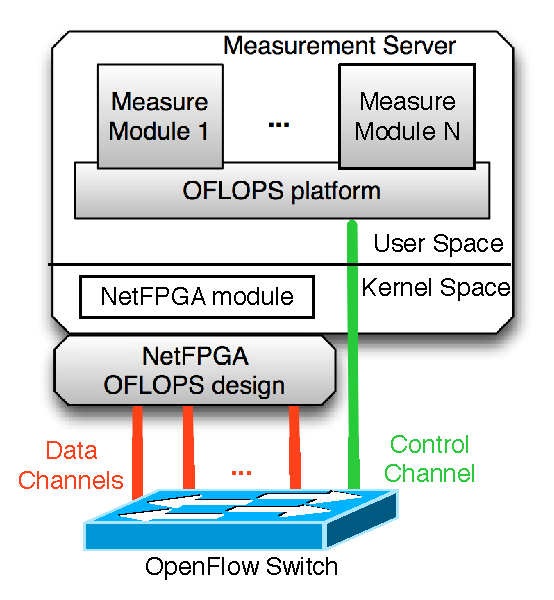
\includegraphics[width=0.30\textwidth]{Chapter1/Chapter1Figs/oflops-design-netfpga}
\label{fig:oflops_design_netfpga}}
\subfigure[Kernel-space]{
  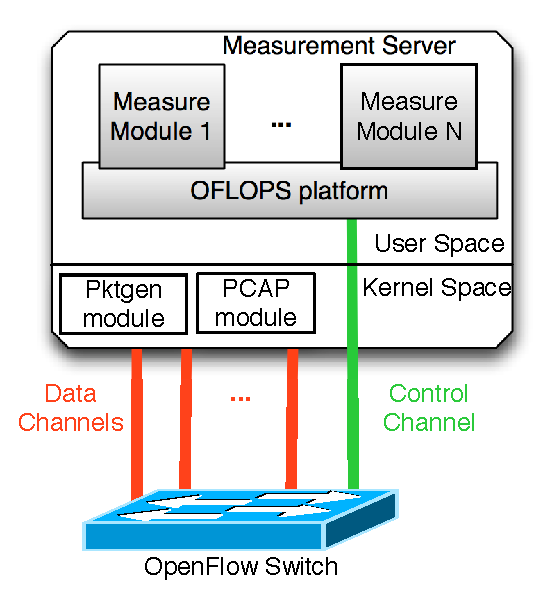
\includegraphics[width=0.30\textwidth]{Chapter1/Chapter1Figs/oflops-design-kernel}
\label{fig:oflops_design_kernel}}
\subfigure[User-space]{
  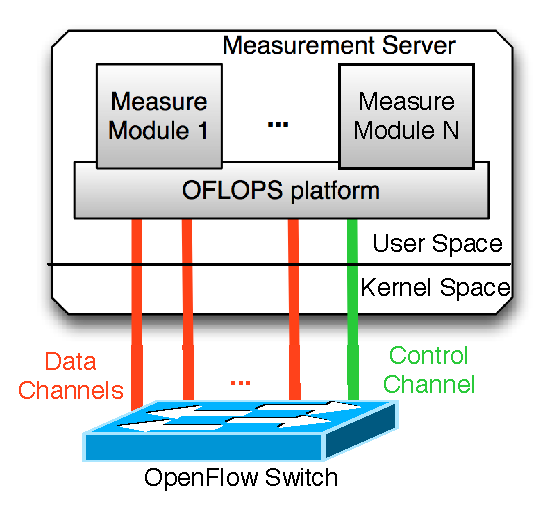
\includegraphics[width=0.30\textwidth]{Chapter1/Chapter1Figs/oflops-design-userspace} 
  \label{fig:oflops_design_userspace}}
\label{fig:oflops_design}
\caption{\oflops measurement setup. The framework provides integration with: 1) a
  high accuracy NetFPGA packet generator hardware
  design~(Figure~\ref{fig:oflops_design_netfpga}), 2) kernel space {\tt pktgen}
  traffic generation module and PCAP packet capturing
  module~\ref{fig:oflops_design_kernel},
  3) User space packet capture and generation
  threads~(Figure~\ref{fig:oflops_design_userspace}} 
\end{figure}

Measuring \of switch implementations is a challenging task in terms of
characterization accuracy, noise suppression and precision.  Performance
characterization is not trivial as most OpenFlow-enabled devices provide rich
functionality but do not disclose implementation details. In order to understand
the performance impact of an experiment, multiple input measurement channels
must be monitored concurrently, such as, data and control channels. Further,
current controller frameworks, like~\cite{Gude08,floodlight}, target production
networks and incur significant measurement noise. Such controllers employ
asynchronous processing libraries and multi-thread execution models, to maximize
the aggregate control channel processing throughput, and provide high-level
programing interfaces, that require multiple data structure allocation and
modification during packet processing.  The processing time of a specific \of
message, especially at high rates, is subject to multiple aspects, like the
thread scheduling policy and the asynchronous library execution
logic~\cite{Jarschel2012}.  Measurement noise suppression in the control plane
requires from the controller framework to minimize message processing and
delegate processing control to the measurement module.  Finally, sub-millisecond
precision in software is subject to unobserved parameters, like OS scheduling
and clock drift. The result of these challenges is that meaningful, controlled,
repeatable performance tests are non-trivial in an \of environment.

The \oflops design philosophy aims to develop a low overhead abstraction layer
that allows interaction with an \of-enabled device over multiple data
channels.  The platform provides a unified system that allows developers to
control and receive information from multiple control sources: data and control
channels as well as SNMP to provide specific switch-state information.
For the development of measurement experiments over \oflops, the platform
provides an event-driven, API that allows developers to handle events
programatically in order to implement and measure custom controller
functionality. The current version is written predominantly in C. Experiments
are compiled as shared libraries and loaded at run-time using a simple
configuration language, through which experimental parameters can be defined.
A schematic of the platform is presented in Figure~\ref{fig:oflops_design}.
Details of the \oflops programming model can be found in the API manual
\cite{oflops-manual}.

The platform is implemented as a multi-threaded application, to take
advantage of modern multicore environments. To reduce latency, our design
avoids concurrent access controls: we leave any concurrency-control complexity 
to individual module implementations. \oflops consists of the following five threads, 
each one serving specific type of events:\\
\textbf{1. Data Packet Generation}: control of data plane traffic generators.\\
\textbf{2. Data Packet Capture}: data plane traffic interception.\\
\textbf{3. Control Channel}: controller events dispatcher.\\
\textbf{4. SNMP Channel}: SNMP event dispatcher.\\
\textbf{5. Time Manager}: time events dispatcher.

\oflops provides the ability to control concurrently multiple data channels to
the switch. Using a tight coupling of the data and control channels, programers
can understand the impact of the measurement scenario on the forwarding plane.
To enable our platform to run on multiple heterogeneous platforms, we have
integrated support for multiple packet generation and capturing mechanisms. For
the packet generation functionality, \oflops supports three mechanisms:
user-space~(Figure~\ref{fig:oflops_design_userspace}), kernel-space through the
pktgen kernel module
module~\cite{pktgen}~(Figure~\ref{fig:oflops_design_kernel}), and
hardware-accelerated through an extension of the design of the NetFPGA Stanford
Packet Generator~\cite{Covington09}~(Figure~\ref{fig:oflops_design_netfpga}).
For the packet capturing and timestamping, the platform supports both the pcap
library and the modified NetFPGA design. Each approach provides different
precisions and different impacts upon the measurement platform.

\begin{figure}
\centering
  \begin{minipage}[b]{0.45\textwidth}
\centering
 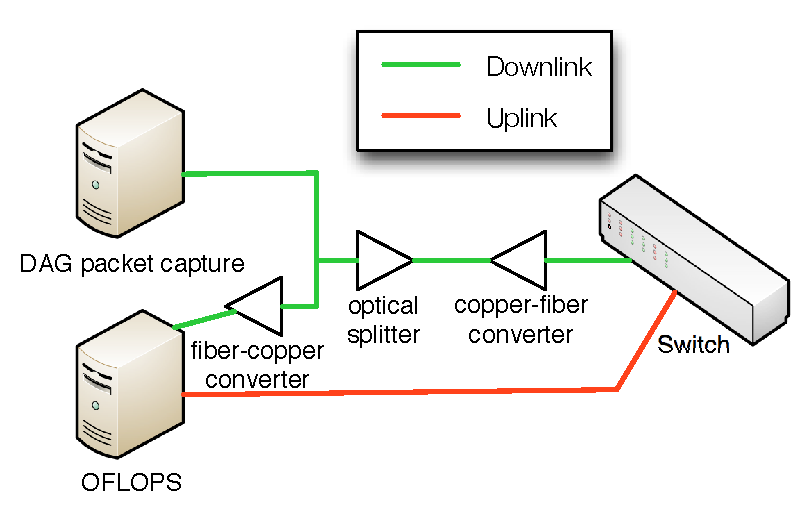
\includegraphics[width=0.99\textwidth]{Chapter1/Chapter1Figs/accuracy-topology} 
 \caption{Measurement topology to evaluate capturing mechanism precision.}
\label{fig:timestamping_topology}
\end{minipage}
\hspace{0.5cm}
  \begin{minipage}[b]{0.45\textwidth}
\centering
 \includegraphics[width=0.99\textwidth]{Chapter1/Chapter1Figs/timer-precision} 
 \caption{Evaluating timestamping precision using a DAG card. PCAP timestamps
   exhibit a significant drift in the order of microseconds, in comparison to
   the NetFPGA hardware design}
\label{fig:timestamping}
\end{minipage}
\end{figure}

In order to assess the accuracy of the traffic capturing mechanism, we use the
topology depicted in Figure~\ref{fig:timestamping_topology} to measure precision
loss in comparison to a DAG card~\cite{dag_card}.  To calculate precision, we
use a constant rate 100 Mbps probe of small packets for a two minute period. The
probe is duplicated, using an optical wiretap with negligible delay, and sent
simultaneously to OFLOPS and to a DAG card. In Figure~\ref{fig:timestamping}, we
plot the differences of the relative timestamp between each OFLOPS timestamping
mechanism and the DAG card for each packet. From the figure, we see that the
PCAP timestamps drift by 6 milliseconds after 2 minutes.  On the other hand, the
NetFPGA timestamping mechanism has a smaller drift at the level of a few
microseconds during the same period.

\section{Measurement Setup}\label{sec:oflops-switches}

At the end of 2009, the \of protocol specification was released in its first
stable version 1.0~\cite{openflow-spec}, the first recommended version
implemented by vendors for production systems.  The switch performance analysis
was contacted in collaboration with T-labs in Spring of 2011. During that
period, the introduction of \of support in commodity switches was limited and
only a small number of devices provided production-level support for the
protocol.  Using \oflops, we evaluated \of-enabled switches from three different
switch vendors.  Vendor 1 provided production-ready \of support, whereas vendors
2 and 3 during that period provided experimental \of support.  The set of
selected switches provided a representative but not exhaustive sample of
available \of-enabled top-of-rack-style switching hardware, during that time.
Details regarding the CPU and the size of the flow table of the switches are
provided in Table~\ref{tbl:switch_list}. In addition the switching fabric in the
vendor hardware specification reports similar non-blocking capacity and packet
processing rates. 

\of is not limited to hardware. The \of protocol reference is the software
switch, \ovs~\cite{openvswitch}, an important implementation for production
environments. Firstly, \ovs provides a replacement for the poor-performing Linux
bridge~\cite{bianco10}, a crucial functionality for virtualised operating
systems.  Currently, the Xen platform uses \ovs to forward traffic between VMs
in the Dum0, a configuration which is inherited by major Cloud providers, like
Amazon and Rackspace.  Secondly, several hardware switch vendors use \ovs as the
basis for the development of their own \of-enabled firmware.  \ovs development
team has standardised a clean abstraction for the control of the packet
forwarding elements (similar to linux HAL), which allows code reuse by any
forwarding entity. Thus, the mature software implementation of the \of protocol
is ported to commercial hardware, making certain implementation bugs less likely
to (re)appear.  We study \ovs alongside our performance and scalability study of
hardware switches. Finally, in our comparison we include the \of switch design
for the NetFPGA platform~\cite{openflow-netfpga}. This implementation is based
on the original \of reference implementation~\cite{of-reference-impl}, extending
it with a hardware forwarding design. 

\begin{table}[h!]
  \begin{center}
  \begin{tabular}{ |c | c | c | }
    \hline                        
    \textbf{Switch} & \textbf{CPU} & \textbf{Flow table size} \\
    \hline  
    Switch1 & PowerPC 500MHz & 3072 mixed flows \\
    \hline  
    Switch2 & PowerPC 666MHz & 1500 mixed flows \\
    \hline  
    Switch3 & PowerPC 828MHz & 2048 mixed flows \\
    \hline  
    \ovs & Xeon 3.6GHz & 1M mixed flows \\
    \hline  
    NetFPGA &  DualCore 2.4GHz & 32K exact \& 100 wildcard \\
    \hline 
  \end{tabular}  
\end{center}
\caption{OpenFlow switch details.}
\label{tbl:switch_list}
\end{table}

In order to conduct our measurements, we setup \oflops on a dual-core 2.4GHz
Xeon server equipped with a NetFPGA card.  For all the experiments we utilize
the NetFPGA-based packet generating and capturing mechanism. 1Gbps control and
data channels are connected directly to the tested switches. We measure the
processing delay incurred by the NetFPGA-based hardware design to be a
near-constant $900$ nsec.

%%%%%%%%%%%%%%%%%%%%%%%%%%%%%%%%%%%%%%%%%%%%%%%
\section{Switch Evaluation}\label{sec:oflops-result}
%%%%%%%%%%%%%%%%%%%%%%%%%%%%%%%%%%%%%%%%%%%%%%%%

% In this section we present a set of tests performed by \oflops to
% measure the behavior and performance of \of-enabled
% devices. These tests target (1) the \of packet processing 
% actions, (2) the update rate of the \of flow table along with 
% its impact on the data plane, (3) the monitoring capabilities provided 
% by \of, and (4) the impact of interactions between different 
% \of operations.

As for most networking standards, there are different ways to implement a given
protocol based on a paper specification. \of is no different in this regard. The
current \of reference implementation is \ovs~\cite{openvswitch}. However,
different software and hardware implementations may not implement all features
defined in the \ovs reference, or they may behave in an unexpected way. In order
to understand the behaviour of switch \of implementation, we develop a suite of
measurement experiments to benchmark the functionality of the elementary
protocol interactions.  These tests target (1) the \of packet processing
actions~(Section~\ref{sec:results-packets}), (2) the packet interception and
packet injection functionality of the
protocol~(section~\ref{sec:results-pktin}), (3) the update rate of the \of flow
table along with its impact on the data plane,~(Section~\ref{sec:results-rate})
(4) the monitoring capabilities provided by
\of~(Section~\ref{sec:results-monitoring}), and (5) the impact of interactions
between different \of operations~(Section~\ref{sec:results-interactions}).


\subsection{Packet Modifications}\label{sec:results-packets}

The \of specification \cite{openflow-spec} defines 10 packet modification
actions which can be applied on incoming packets. Available actions include
modification of source and destination MAC and IP addresses, VLAN tag and PCP
fields and TCP and UDP source and destination port numbers. The action list
of a flow definition can contain any combination of them. The left column of
Table~\ref{tbl:feature_delay} lists the packet fields that can be modified by an
\of-enabled switch.  These actions are used by network devices such as IP
routers (e.g., rewriting of source and destination MAC addresses) and NAT
(rewriting of IP addresses and ports). Existing network equipment is tailored to
perform a subset of these operations, usually in hardware to sustain line rate.
% On the other hand, how these operations are to be used is yet to be defined for
% new network primitives and applications, such as network virtualization,
% mobility support, or flow-based traffic engineering.

% Explain how we measure the time taken to perform the modification.
To measure the time taken by an \of switch to modify a packet field header, we
generate from the NetFPGA card UDP packets of 100 bytes at a constant rate of
100Mbps (approximately 125 Kpps).  This rate is high enough to give
statistically significant results in a short period of time, without causing
packet queuing.  The flow table is initialized with a flow that applies a
specific action on all probe packets and the processing delay is calculated as
the difference between the transmission and receipt timestamps provided by the
NetFPGA.  We report in Table~\ref{tbl:feature_delay} the median processing delay
for each action, along with its standard deviation, and the percent of lost
packets of the measurement probe.

\begin{table*}[tb]
\begin{flushleft}
        \begin{tabular}[t]{ |l | c | c | c || c | c | c  || c | c | c | }
          \hline                       
          Mod. type & \multicolumn{3}{|c|}{Switch 1} & \multicolumn{3}{|c|}{ovs} &
          \multicolumn{3}{|c|}{Switch 2} \\ 
          \hline                       
          & med & sd & loss\%  & med & sd & loss\% & med & sd & loss\%\\
          \hline  
          Forward & 4 & 0 & 0 & 35 & 13 & 0& 6 & 0 & 0 \\
          \hline  
          MAC addr. & 4 & 0 & 0 & 35 & 13 & 0& 302 & 727 & 88\\
          \hline  
          IP addr. & 3 & 0 & 0 & 36 & 13 & 0 & 302 & 615 & 88\\
          \hline  
          IP ToS & 3 & 0 & 0 & 36 & 16 & 0 & 6 & 0 & 0\\
          \hline  
          L4 port & 3 & 0 & 0 & 35 & 15 & 0 & 302 & 611 &  88\\
          \hline  
          VLAN pcp & 3 & 0 & 0 & 36 & 20 & 0 & 6 & 0 & 0\\
          \hline  
          VLAN id & 4 & 0 & 0 & 35 & 17 & 0 & 301 & 610 & 88\\
          \hline  
          VLAN rem. & 4 & 0 & 0 & 35 & 15 & 0 & 335 & 626 & 88\\
      \hline
    \end{tabular}
   \begin{tabular}[t]{ |l | c | c | c || c | c | c | }
          \hline                       
          Mod. type & \multicolumn{3}{|c|}{Switch 3} & \multicolumn{3}{|c|}{NetFPGA}\\ 
          \hline                       
          & med & sd & loss\%  & med & sd & loss\% \\
          \hline  
          Forward & 5 & 0 & 0 & 3 & 0 & 0 \\
          \hline  
          MAC addr. & - & - & 100 & 3 & 0 & 0 \\
          \hline  
          IP addr. & - & - &  100 & 3 & 0 & 0 \\
          \hline  
          IP ToS & - & - & 100 & 3 & 0 & 0 \\
          \hline  
          L4 port & - & - & 100 & 3 & 0 & 0 \\
          \hline  
          VLAN pcp & 5 & 0 & 0 & 3 & 0 & 0 \\
          \hline  
          VLAN id & 5 & 0 & 0 & 3 & 0 & 0  \\
          \hline  
          VLAN rem. & 5 & 0 & 0 & 3 & 0 & 0 \\
      \hline
    \end{tabular}
 
\caption{Time in $\mu$s to perform individual packet modifications and packet
loss. Processing delay indicates whether the operation is
  implemented in hardware (\textless10$\mu$s) or performed by the CPU (\textgreater10$\mu$s).}
  \label{tbl:feature_delay}
\end{flushleft}
\end{table*}
% What the table shows...

We observe significant differences in the performance of the hardware switches
due in part to the way their firmware implements packet modifications. Switch1,
with its production-grade implementation, handles all modifications in hardware;
this explains its low packet processing delay between 3 and 4 microseconds. On
the other hand, Switch2 and Switch3 each run experimental firmware that
provided, at the time, only partial hardware support for \of actions. Switch2
uses the switch CPU to perform some of the available field modifications,
resulting in two orders of magnitude higher packet processing delay and
variance.  Switch3 follows a different approach; all packets of flows with
actions not supported in hardware are silently discarded. The performance of the
\ovs software implementation lies between Switch1 and the other hardware
switches.  \ovs fully implements all \of actions. However, hardware switches
outperform \ovs when the flow actions are supported in hardware.

We conducted a further series of experiments with variable numbers of packet
modifications in the flow action list. We observed, that the combined processing
time of a set of packet modifications is equal to the highest processing time
across all individual actions in the set (e.g.~Switch2 requires approximately
300~msec per packet to modify both IP source addresses and IP ToS field).
Furthermore, we notice that for Switch1 and \ovs there is a limit of 7
actions, which exposes limits enclosed in the implementation.

\subsection{Traffic Interception and Injection}\label{sec:results-pktin}

\begin{figure}[ht]
  \begin{center}
    \subfigure[{\tt packet\_in} message latency]
    {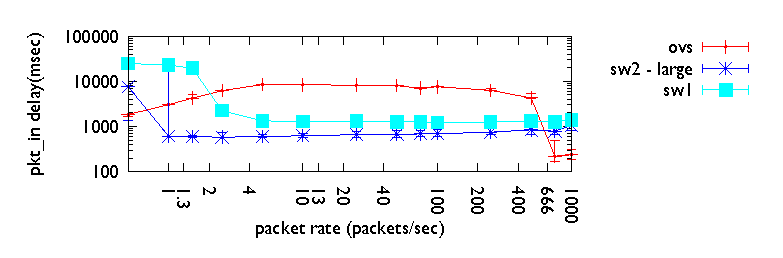
\includegraphics[width=0.99\textwidth]{pkt_in_delay}}
    \subfigure[{\tt packet\_out} message latency]
	{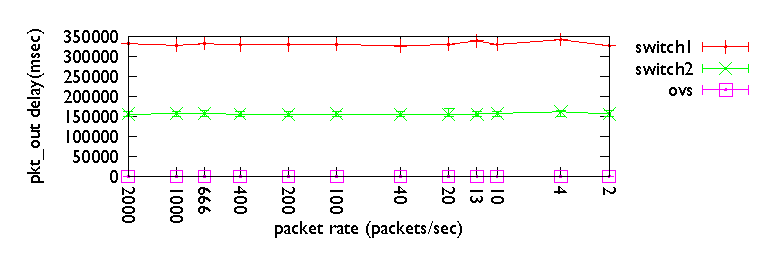
\includegraphics[width=0.99\textwidth]{pkt_out_delay}}
  \end{center}
  \caption{Latency to intercept and inject a packet using the \of protocol}
  \label{fig:pkt_in_out_delay}
\end{figure}

\of protocol permits a controller to intercept or inject traffic from the
control plane. Packet interception is fundamental for reactive control applications, while
packet injection enables control application interaction with network hosts.
Nonetheless, the interception mechanism in \of has been characterised as a
significant bottleneck for the control plane in early \of protocol
deployments~\cite{Kobayashi:vn}. This is a direct consequence of the silicon
design in current \of switches, that develop such functionality over a
low-bandwidth exception-notification
channel~(Section~\ref{sec:background:forwarding}). In order to characterise these
functionalities, we design two simple experiments. For packet interception, we
remove all entries from the switch flow table and send a measurement probe of
small packets (100 bytes) on one of the data channels. We measure the delay
between the time the packet was transmitted on the data channel and the time the
controller received the equivalent {\tt packet\_in} message. For packet
injection, we transmit {\tt packet\_out} messages over the control channel and
measure the delay to receive the packet on a data channel. In
Figure~\ref{fig:pkt_in_out_delay}, we plot the median packet processing latency
for {\tt packet\_in} and {\tt packet\_out} messages. We omit in this experiment
Switch 3 as these functionalities incur high CPU utilisation and, after a few
seconds of traffic, the control channel becomes unresponsive. For {\tt
  packet\_out} messages, all implementations rate limit their transmission
through the TCP advertised window of the control connection and as a result the
latency is near constant. We observe that hardware switch exhibit high latency
(150 msec for Switch2 and 350 msec for Switch1), in comparison to \ovs
(approximately 0.1 msec).  For {\tt packet\_in} messages, we observe diverse
behaviours between hardware switches at high packet rates. For Switch1, packet
loss and latency becomes note-worthy beyond 400 packets/sec, while the switch
can process up to 500 packets/sec. For Switch2 latency and packet loss are
significantly lower and stable. Switch2 incurs high processing latency beyond
2000 packets/sec.  \ovs, has a high but stable latency for any tested
data rates. 

\subsection{Flow Table Update Rate}\label{sec:results-rate}

The flow table is a central component of an \of switch and is the
equivalent of a Forwarding Information Base (FIB) on routers. Given the
importance of FIB updates on commercial routers, e.g., to reduce the impact of
control plane dynamics on the data plane, the FIB update processing time of
commercial routers provide useful reference points and lower bounds for the time
to update a flow entry on an \of switch. The time to install a new entry on
commercial routers has been reported in the range of a few hundreds of
microseconds~\cite{shaikh-igp}.

\of provides a mechanism to define barriers between sets of commands: the
\texttt{barrier} command. According to the OpenFlow
specification~\cite{openflow-spec}, the \texttt{barrier} command is a way to be
notified that a set of \of operations has been completed. Further, the switch
has to complete the set of operations issued prior to the \texttt{barrier}
before executing any further operation. If the \of implementations comply with
the specification, we expect to receive a \texttt{barrier} notification for a
flow modification once the flow table of the switch has been updated, implying
that the change can be seen from the data plane.

We check the behavior of the tested \of implementations, finding variation among
them. For \ovs and Switch1, Figure~\ref{fig:flow_insertion_comparison} shows the
time to install a set of entries in the flow table. Switch2 and Switch3 are not
reported as this \of message is not supported by the firmware.  For this
experiment, \oflops relies on a stream of packets of 100 bytes at a constant
rate of 100 Kpackets/sec (10Mbps) that targets the newly installed flows in a
round-robin manner. The probe achieves sufficiently low inter-packet periods in
order to accurately measure the flow insertion time.
%With such a probe stream, we obtain an inter-packet
%period of less than 100$\mu$s, adequate for measuring any change in
%the flow-insertion time.
% 100 bytes -> 1 packet
% 10^7 bytes -> x => x = 10^5 = 100 K

\begin{figure}[ht]
  \begin{center}
    \subfigure[\ovs (log-log scale)]
    {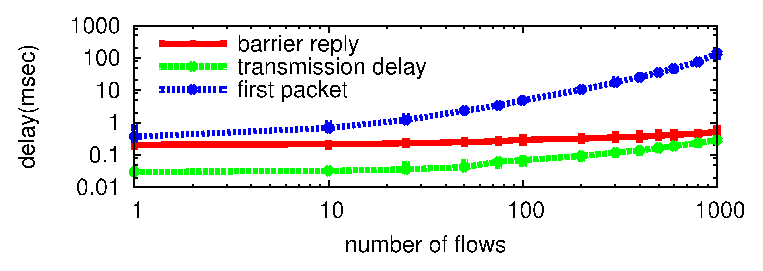
\includegraphics[width=0.99\textwidth]{openvswitch_mod_flow_exact_comparison}}
    \subfigure[Switch1 (log-log scale)]
	{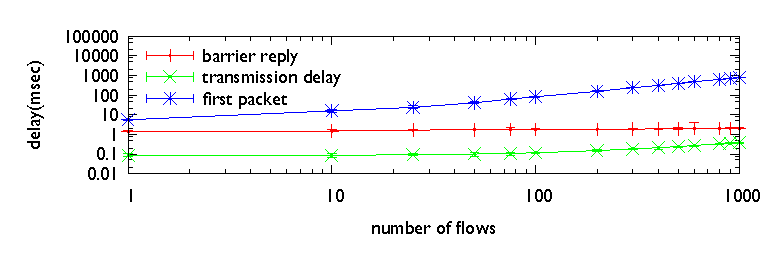
\includegraphics[width=0.99\textwidth]{nec_mod_flow_exact_comparison}}
  \end{center}
  \caption{Flow entry insertion delay: as reported using the
    \texttt{barrier} notification and as observed at the data
    plane.}
  \label{fig:flow_insertion_comparison}
\end{figure}


In Figure~\ref{fig:flow_insertion_comparison}, we show three different times.
The first, {\it barrier notification}, is derived by measuring the time between
when the \textbf{first insertion command} is sent by the \oflops controller and
the time the \texttt{barrier} notification is received by the PC. The second,
{\it transmission delay}, is the time between the first and last flow insertion
commands are sent out from the PC running \oflops.  The third, {\it first
  packet}, is the time between the \textbf{first insertion command} is issued
and a packet has been observed for the last of the (newly) inserted rules. For
each configuration, we run the experiment 100 times and
Figure~\ref{fig:flow_insertion_comparison} shows the median result as well as
the $10^{th}$ and $90^{th}$ percentiles, although the variations are small and
cannot be easily viewed.
%\todo{point that the error
%  bounds are tight and cannot easily viewed on the graph}

From Figure~\ref{fig:flow_insertion_comparison}, we observe that even though the
{\it transmission delay} for sending flow insertion commands increases with
their number, this time is negligible when compared with data plane measurements
({\it first packet}). Notably, the {\it barrier notification} measurements are
almost constant, increasing only as the transmission delay increases (difficult
to discern on the log-log plot) and, critically, this operation returns before
any {\it first packet} measurement. This implies that the way the {\it barrier
  notification} is implemented does not reflect the time when the hardware
flow-table has been updated.

In these results we demonstrate how \oflops can compute per-flow overheads. We
observe that the flow insertion time for Switch1 starts at $1.8$ms for a single
entry, but converges toward an approximate overhead of $1$ms per inserted entry
as the number of insertions grows.

%%%%%%%%%%%%%%%%%%%%%%%%%%%%%%%%%%%%%%%%%%%%%%
\subsubsection*{Flow insertion types}
%%%%%%%%%%%%%%%%%%%%%%%%%%%%%%%%%%%%%%%%%%%%%%

\begin{figure}[h]
  \begin{center}
    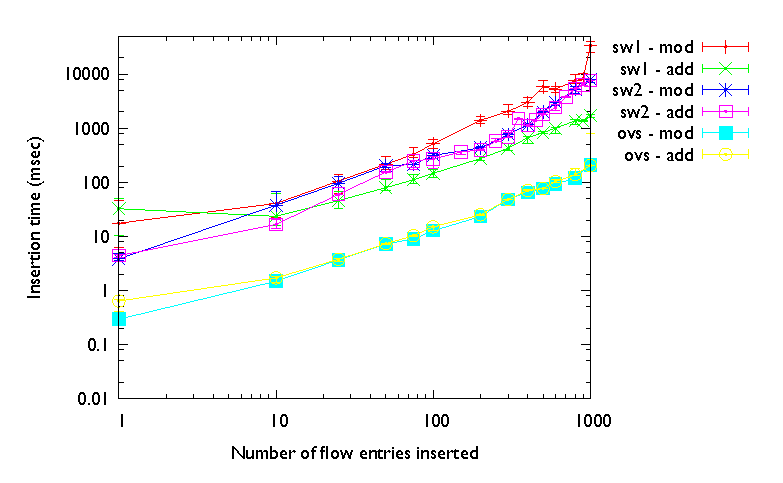
\includegraphics[width=0.80\textwidth]{flow_insertion_delay}
  \end{center}
  \caption{Delay of flow insertion and flow modification, as observed
    from the data plane (log-log scale).}
  \label{fig:flow_insertion_delay}
\end{figure}

We now distinguish between flow insertions and the modification of existing
flows.  With \of, a flow rule may perform exact packet matches or use
wild-cards to match a range of values. Figure~\ref{fig:flow_insertion_delay}
compares the flow insertion delay as a function of the number of inserted
entries. This is done for the insertion of new entries and for the modification
of existing entries.

These results show that for software switches that keep all entries in memory,
the type of entry or insertion does not make a difference in the flow insertion
time.  Surprisingly, both Switch1 and Switch2 take more time to modify existing
flow entries compared to adding new flow entries.  For Switch1, this occurs for
more than 10 new entries, while for Switch2 this occurs after a few tens of new
entries.  After discussing this issue with the vendor of Switch2, we came to the
following conclusion: as the number of TCAM entries increases, updates become
more complex as they typically requires re-ordering of existing entries.
In~\cite{Gupta01}, the authors characterise the update complexity of a TCAM to
be linear. 

Clearly, the results depend both on the entry type and implementation.  For
example, exact match entries may be handled through a hardware or software hash
table. Whereas, wild-carded entries, requiring support for variable length
lookup, must be handled by specialized memory modules, such as a TCAM. With such
possible choices and range of different experiments, the flow insertion times
reported in Figure~\ref{fig:flow_insertion_delay} are not generalizable, but
rather depend on the type of insertion entry and implementation.

% %%%%%%%%%%%%%%%%%%%%%%%%%%%
\subsection{Flow Monitoring}\label{sec:results-monitoring}
% %%%%%%%%%%%%%%%%%%%%%%%%%%%

The use of OpenFlow as a monitoring platform has already been suggested for the
applications of traffic matrix computation~\cite{opentm-pam,tm-presto} and
identifying large traffic aggregates~\cite{openflow-measurement-hotice}. To
obtain direct information about the state of the traffic received by an OpenFlow
switch, the OpenFlow protocol provides a mechanism to query traffic statistics,
either on a per-flow basis or across aggregates matching multiple flows and
supports packet and byte counters. 
%The result of a query returns packet and byte
%counters, either for the matched flows individually or for the
%aggregate.

We now test the performance implications of the traffic statistics reporting
mechanism of \of. Using \oflops, we install flow entries that match packets sent
on the data path. Simultaneously, we start sending flow statistics requests to
the switch. Throughout the experiment we record the delay getting a reply for
each query, the amount of packets that the switch sends for each reply and the
departure and arrival timestamps of the probe packets.

Figure~\ref{fig:stat_request_latency} reports the time to receive a flow
statistics reply for each switch, as a function of the request rate. Despite the
rate of statistics requests being modest, quite high CPU utilization is recorded
for even a few queries per second being sent. Figure~\ref{fig:stat_request_cpu}
reports the switch-CPU utilization as a function of the flow statistics
inter-request time. Statistics are retrieved using SNMP. Switch3 is excluded for
lack of SNMP support.

\begin{figure}[h]
  \begin{center}
    \subfigure[Reply time.]
    {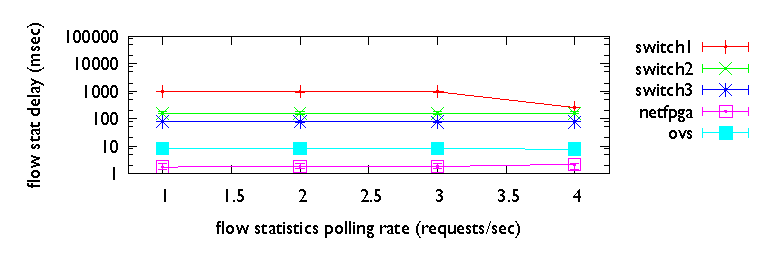
\includegraphics[width=0.99\textwidth]{flow_stats_delay} \label{fig:stat_request_latency}}
    \subfigure[CPU utilization.]
      {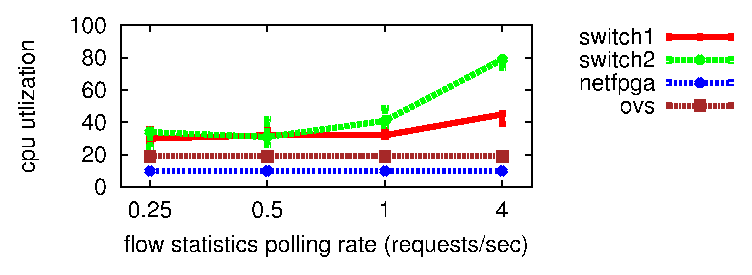
\includegraphics[width=0.99\textwidth]{flow_stats_cpu}\label{fig:stat_request_cpu}}
  \end{center}
  \caption{Time to receive a flow statistic (median) and corresponding CPU utilization.}
  \label{fig:stat_request}
\end{figure}

From the flow statistics reply times, we observe that all switches have
(near-)constant response delays: the delay itself relates to the type of switch.
As expected, software switches have faster response times than hardware
switches, reflecting the availability of the information in memory without the
need to poll multiple hardware counters. These consistent response times also
hide the behavior of the exclusively hardware switches whose CPU time increases
proportionally with the rate of requests.  We observe two types of behavior from
the hardware switches: the switch has a high CPU utilization, answering
flow-stats requests as fast as possible (Switch2), or the switch delays
responses, avoiding over-loading its CPU (Switch1). Furthermore, for Switch1, we
notice that the switch is applying a pacing mechanism on its replies.
Specifically, at low polling rates the switch splits its answer across multiple
TCP segments: each segment containing statistics for a single flow.  As the
probing rate increases, the switch will aggregate multiple flows into a single
segment. This suggests that independent queuing mechanisms are used for handling
flow statistics requests. Finally, neither software nor NetFPGA switches see an
impact of the flow-stats rate on their CPU, thanks to their significantly more
powerful PC CPUs (Table~\ref{tbl:switch_list}).

%%%%%%%%%%%%%%%%%%%%%%%%%%%%%%%%%%%%%%%%%
\subsection{\of Command Interaction}\label{sec:results-interactions}
%%%%%%%%%%%%%%%%%%%%%%%%%%%%%%%%%%%%%%%%%

% why is it important this experiment

An advanced feature of the \of protocol is its ability to provide network
control applications with, e.g., flow arrival notifications from the network,
while simultaneously providing fine-grain control of the forwarding process.
This permits applications to adapt in real time to the requirements and load of
the network~\cite{plug_n_serv,Yap09}. Using \oflops advanced measurement
instrumentation, we develop a test scenario of dynamic network control, in order
to understand the behavior of the switch control and data plane.  In this
scenario, we emulate the simultaneous querying of traffic statistics and
modification of the flow table.  More specifically, we extend
Section~\ref{sec:results-rate} by showing how the mechanisms of traffic
statistics extraction and table manipulation interact. Specifically, we
initialize the flow table with 1024 exact match flows and measure the delay to
update a subset of 100 flows.  Simultaneously, the measurement module polls the
switch for full table statistics at a constant rate. The experiment uses a
constant rate 10Mbps packet probe to monitor the data path, and polls every 10
seconds for SNMP CPU values.

\begin{figure}[t]
  \begin{center}
    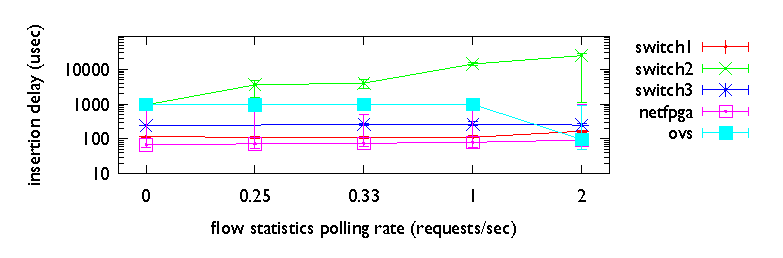
\includegraphics[width=0.99\textwidth]{interaction_test}
  \end{center}
  \caption{Delay when updating  flow table while the controller polls
    for statistics.}
  \label{fig:interaction_test}
\end{figure}

In this experiment, we control the probing rate for the flow statistics
extraction mechanism, and we plot the time necessary before the modified flows
become active in the flow table. For each probing rate, we repeat the experiment
50 times, plotting the median, $10^{th}$ and $90^{th}$ percentile. In
Figure~\ref{fig:interaction_test} we can see that, for lower polling rates,
implementations have a near-constant insertion delay comparable to the results
of Section~\ref{sec:results-rate}.  For higher probing rates on the other hand,
Switch1 and Switch3 do not differ much in their behavior. In contrast, Switch2
exhibits a noteworthy increase in the insertion delay. This is explained by the
CPU utilization increase incurred by the flow statistics polling
(Figure~\ref{fig:stat_request_cpu}). Finally, \ovs exhibits a marginal decrease
in the median insertion delay and at the same time an increase in its variance.
We believe this behavior is caused by interactions with the OS scheduling
mechanism: the constant polling causes frequent interrupts for the user-space
daemon of the switch, which leads to a batched handling of requests.

% LocalWords:  OpenFlow Oflops IP VLAN balancers SDNs virtualization NetFPGA th
% LocalWords:  UDP Mbps Gbps multiport timestamp \ovs dev dest src addr
% LocalWords:  NIC ToS TCP pcp interpacket TCAM lookup SNMP CPUs parameterising

\section{\of Macro-experimentation} \label{sec:sdnsim-intro}

% SDN paradigm provides functional evolution in a network that is backward
% compatible with existing network systems. The evolution is achieved through
% network control distribution to external programmable units. In order to have 
% effective control delegation, an SDN protocol
% \textit{must} provide sufficient forward plane control and feedback to the 
% controlling entity. So far the trend in \of design is to aggregate control in a single
% control unit, in order to have a single point of control in the network. This
% aggregation permits on one hand to achieve higher optimality in forwarding
% policy, while on the other hand the logic can be developed in richer programming
% environments, than the embedded systems usually found in current network
% devices.

\oflops, along with Cbench~\cite{cbench}, provides a sufficient toolchain to
profile functionality of \of building blocks.  Nonetheless, in order to
understand the impact of scalable control in a computer network, we require
mechanisms to transform \of building block performance profiles into
network-wide performance measurements, under specific traffic patterns and
network topology.  A common practice to reason about performance and correctness
of a network architecture relies on the design of experiments that reproduce
specific network-wide functionalities.  In the related literature on network
experimentation there have been two main implementation approaches : {\it
  realistic-testbed} and {\it simulation}.

Realistic testbeds reproduce in full detail the properties of the deployment
environment. They provide an optimal measurement environment with complete
control over the parameter of the experiment and optimal time scalability.
Nonetheless, realistic testbeds incur significant resource and configuration
overhead, which scale sub-optimally with respect to the experiment size.  For
example, setting up a realistic testbed for datacenter network experimentation
requires a significant number of machines and network devices, careful
interconnection planning and targeted metrication and analysis of the resulting
system. In an effort to improve resource scalability for realistic testbeds, the
research community provides a number of shared testbeds. Shared testbeds employ
techniques such as virtualization and statistical multiplexing to scale
resource utilization in a multi-tenant experimentation
platform~\cite{planetlab,emulab}.  However, shared testbeds are not always a
good fit for network experiments. In such testing environments, there is limited
resource control, while resource sharing may introduce measurement noise, which
is not always detectable and removable. 

In the simulation approach, researchers replace parts of the functionality of
the system with simplified models~\cite{Varga2008,issariyakul2012}.  Simulation
reduces the complexity of large scale network experiments, and provides resource
scalability. Nonetheless, the scaling property has inherent limitations.
Firstly, the fidelity of the results depends greatly on the validity of the
model assumptions. Secondly, in order to simulate network experiments, users
usually need to readjust the logic of their experiments to fit with the
abstraction of the underlying models.  For example, POSIX socket-based
applications must modify their connection abstraction to match the API of the
simulation platform, while forwarding plane traffic patterns may have to
transform into stochastic models. 

\sdnsim\footnote{\sdnsim is under the GPL licence and can be downloaded from
  \url{http://github.com/crotsos/sdnsim/}} is a novel network experimentation
framework, that bridges the two aforthmentioned approaches. The framework is
written in OCaml, a high performance functional language, and extends the
functionality of the Mirage~\footnote{\mirageurl} library OS. Developers can
describe network functionality over the \mirage OS abstraction, and
at compilation transform the experiment definition in a concrete experiment
realisation.  \sdnsim provides two experimentation options: \emph{Simulation},
transforms the experiment definition into an \ns{3}~\cite{Henderson2006}
simulation, and \emph{Emulation}, translates the experiment definition in
Xen-based emulation of the experiment.

\section{Mirage Library OS} \label{sec:mirage-intro}

% \begin{figure}
% 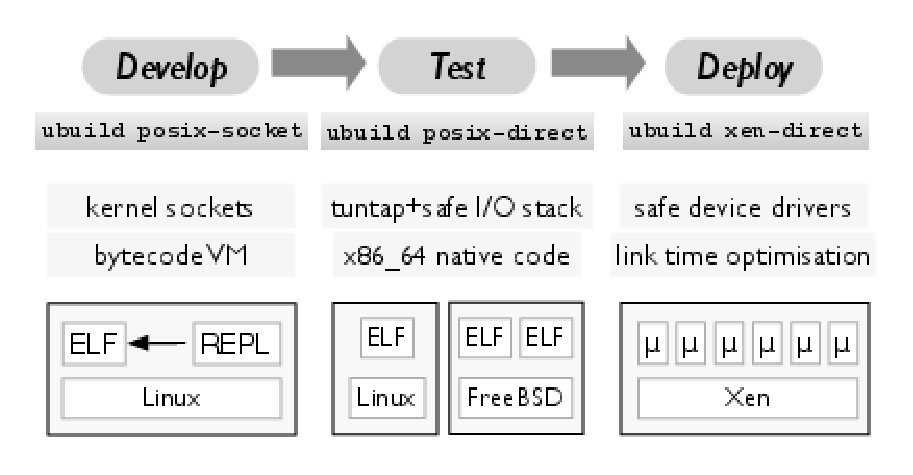
\includegraphics[width=0.9\textwidth]{mirage-toolchain}
% \caption{Specialising a \mirage application through recompilation alone, from
%   interactive UNIX Read-Eval-Print Loop, to reduce dependency on the host
%   kernel, and finally a unikernel VM.}
% \label{fig:mirage-toolchain}
% \end{figure}

% Cloud computing has revolutionized the way the business use IT infrastructures
% as well as the way we develop distributed computing applications. The
% abstraction is straightforward. A third party entity takes responsibility to
% maintain a datacenter. This infrastructure, is partitioned into smaller virtual
% computational units which clients can rent in order to run their applications.
% The elegance of this model is based on simplicity of the abstraction that the
% cloud provider provides to the user and the ability to port existing services
% running on a personal computer or a server to the cloud platform. 

% Although the simplicity of the exposed abstraction, the cloud architecture
% consist of a complex set of processing layers. A single application VM would
% include: i) the virtualization runtime layer, ii) the guest OS kernel layer,
% iii) A language runtime layer (POSIX, JVM etc.) iv) user-space
% thread layer. This layer complexity, although it provides excellent backwards
% compatibility for existing datacenter applications, it makes the process of
% optimisation, debugging as well as security difficult, while there is a
% significant overlap on the functionality provided by each layer. 

% todo{why do I use \mirage?}
% \begin{itemize}
%   \item Simple abstraction that can translate to any backend.
%   \item Provides all the required functionality.
%   \item Network layer doesn't incur complexity that can change logic.
%   \item very low memory CPU requirement by the platform. 
% \end{itemize}
\begin{table}
\centering
\begin{tabular}{@{\extracolsep{0pt}}l|c}
\emph{Appliance} & \emph{Binary size (MB)} \\ 
\hline
DNS & 0.184 \\
Web Server & 0.172 \\
OpenFlow switch & 0.164 \\
OpenFlow controller & 0.168 \\
\end{tabular}
\caption{\label{t:codesize}Sizes of Mirage application images. Configuration and
  data are compiled directly into the image.}
\end{table}

% One of the core goals of the \sdnsim platform is to establish a simple
% abstraction over which a developer can describe an experimentation scenario.  At
% compile time the framework translates the experiment description into a concrete
% implementation which emulates or simulates the scenario.  Mirage is a
% cloud service development framework which revisits the idea of library OSes, in
% an effort to improve performance, scalability and security.  Mirage applications
% are single purpose appliances that are compile-time specialised into standalone
% kernels deployable on the Xen platform.  

In \sdnsim we use the Mirage framework to provide an application development
environment. Mirage is a a cloud-service development framework written
predominantly in OCaml, where applications are single purpose appliances that
are compile-time specialised into standalone kernels deployable on the Xen
platform.  We chose to use rhe Mirage framework due to two fundamental
functional properties: low memory footprint and simplified integratability.
Mirage revisits the idea of library OS; OS functionality is separated into
logical modules and added to an appliance only if the code expresses an explicit
dependency.  As a result, a Mirage application will integrate in a VM only the
required OS functionality, resulting in compact OS images with minimized
memory requirements. In Table~\ref{t:codesize}, we present the compiled image
size for a set of Mirage applications.

Furthermore, Mirage OS provides a simple development API for systems
programming. This functionality is implemented by two core modules, named
\textit{Net} and \textit{OS}.  The OS module provides basic thread scheduling,
device management and device IO functionality, while the Net module provide a
network stack supporting ICMP, IP, TCP, UDP and DHCP protocols through a socket-like
programming API. The interface of the core Mirage API is sufficiently generic to
enable development of complex distributed services, while sufficiently simple to
integrate Mirage functionality over a wide range of platforms. Specifically, a
Mirage application can compile into a Xen image, a linux application and a
nodeJS executable. Currently, the platform is also ported to the FreeBSD kernel
space and the BareMetal OS~\cite{baremetalOS}, a high performance assembly-code
OS.

\section{\sdnsim design} \label{sec:sdnsim-design}

\lstset{language=XML,
numberstyle=\footnotesize,
basicstyle=\ttfamily\footnotesize,
captionpos=b,
}
\begin{lstlisting}[caption={A sample \sdnsim configuration file interconnecting
  a server and a client host},label={lst:sdnsim-conf}]
<?xml version="1.0" encoding="ISO-8859-1"?>
<topology module="Simple_tcp_test" backend="ns3-direct" 
    duration="30">
  <modules>
    <library>lwt</library>
    <library>lwt.syntax</library>
    <library>cstruct</library>
    <library>cstruct.syntax</library>
    <library>mirage</library>
    <library>mirage-net</library>
    <library>pttcp</library>
  </modules>
  <node name="host1" main="host_inner"> 
    <param>1</param>
  </node>
  <node name="host2" main="host_inner"> 
    <param>2</param>
  </node>
  <link src="host1" dst="host2" delay="10" rate="100" 
    queue_size="100" pcap="false"/>
  <link_ext host="host1" dev="eth1" delay="10" rate="100" 
    queue_size="100" pcap="false" ip="10.1.1.1">
</topology>
\end{lstlisting}

From the developer perspective, \sdnsim consists of a single executable that
functions as an OCaml build system. Developers implement host functionality as
Mirage applications, and use a single XML file to describe the network topology
and assign functionality to network nodes.  A sample XML file is presented in
Listing~\ref{lst:sdnsim-conf}. The configuration describes a simple client
(host1) - server (host2) configuration.  A minimum experiment definition must
define the core code module~(topology@module), the target
executable~(topology@backend) and the duration of the
experiment~(topology@duration). In order to define a host, \sdnsim uses a host
XML entity. Each host entity must define a host name~(node@name) and a host main
function~(node@main), while a number of named parameters~(node/param) can be
passed to the main function. The link XML entity defines a link between two
hosts~(link@src, link@dst) along with the device~(link@queue\_size, link@pcap)
and propagation properties~(link@rate, link@delay), using the link XML entity.
Finally, links can also be used to integrate external network interfaces into
the simulation, in order to allow the experiment to interact with applications
outside of the experiment scope. We enable this functionality using the
link\_ext XML entity which is similar to the link entity, but instead of src and
destination attributes, it uses the host and dev entities to define the host to
which the entity will be attached. In addition, an ip attribute is used to
define the address of the device. 

The functionality of a node in the \sdnsim platform can be split in 3 layers.  A
simple representation of the architecture of an \sdnsim host is depicted in
Figure~\ref{fig:sdnsim-arch}.  The top layer contains the application logic of
the host. This layer is defined by the developer and encodes the traffic model
and the network forwarding logic of the experiment. In order to allow realistic
traffic patterns, \sdnsim reuses all the application libraries
supported by the \mirage platform, reported in Table~\ref{t:facilities}. In addition,
we modify the \of processing code and introduce a latency control mechanism. 
Using the rate control mechanism, \sdnsim can simulate and emulate
switch and controller models, measured through the \oflops and Cbench tools.
We also have implemented in OCaml the pttcp tcp test tool~\cite{pttcp} for
model driven traffic generation. 

The middle layer of the host architecture, contains the network and the OS
libraries of the Mirage platform. This layer provides OS functionality to the
application layer. Finally, the lower layer of the host architecture, provides
integration of the Mirage OS with the execution environment of the experiment.
Currently, \sdnsim supports two execution environments: the {\it \ns{3}}
\/simulation platform  and the {\it Xen} \/virtualisation platform. These two
execution environments are highly heterogeneous and employ different execution
models.  In the rest of this section we present details on the integration of
\sdnsim experiments with each execution environment.  Since \sdnsim aims for
high network accuracy, we focus our presentation on how integration occur on
network functionality and time.

\begin{table}
\centering
\begin{tabular}{r|p{0.6\columnwidth}}
\emph{Subsystem} & \emph{Implemented Protocols} \\
\hline 
% Core        & Lwt, Cstruct, Regexp, UTF8, Cryptokit \\
Network     & Ethernet, ARP, DHCP, IPv4, ICMP, UDP, TCP, OpenFlow\\ 
Storage     & Simple key-value, FAT-32, Append B-Tree, Memcache \\
Application & DNS, SSH, HTTP, XMPP, SMTP  \\ 
Formats     & JSON, XML, CSS, S-Expressions\\
\end{tabular}
\caption{\label{t:facilities}System facilities provided as \mirage{}
        libraries.}
\end{table}

\begin{figure}[ht] 
\centering
\subfigure[\ns{3}]{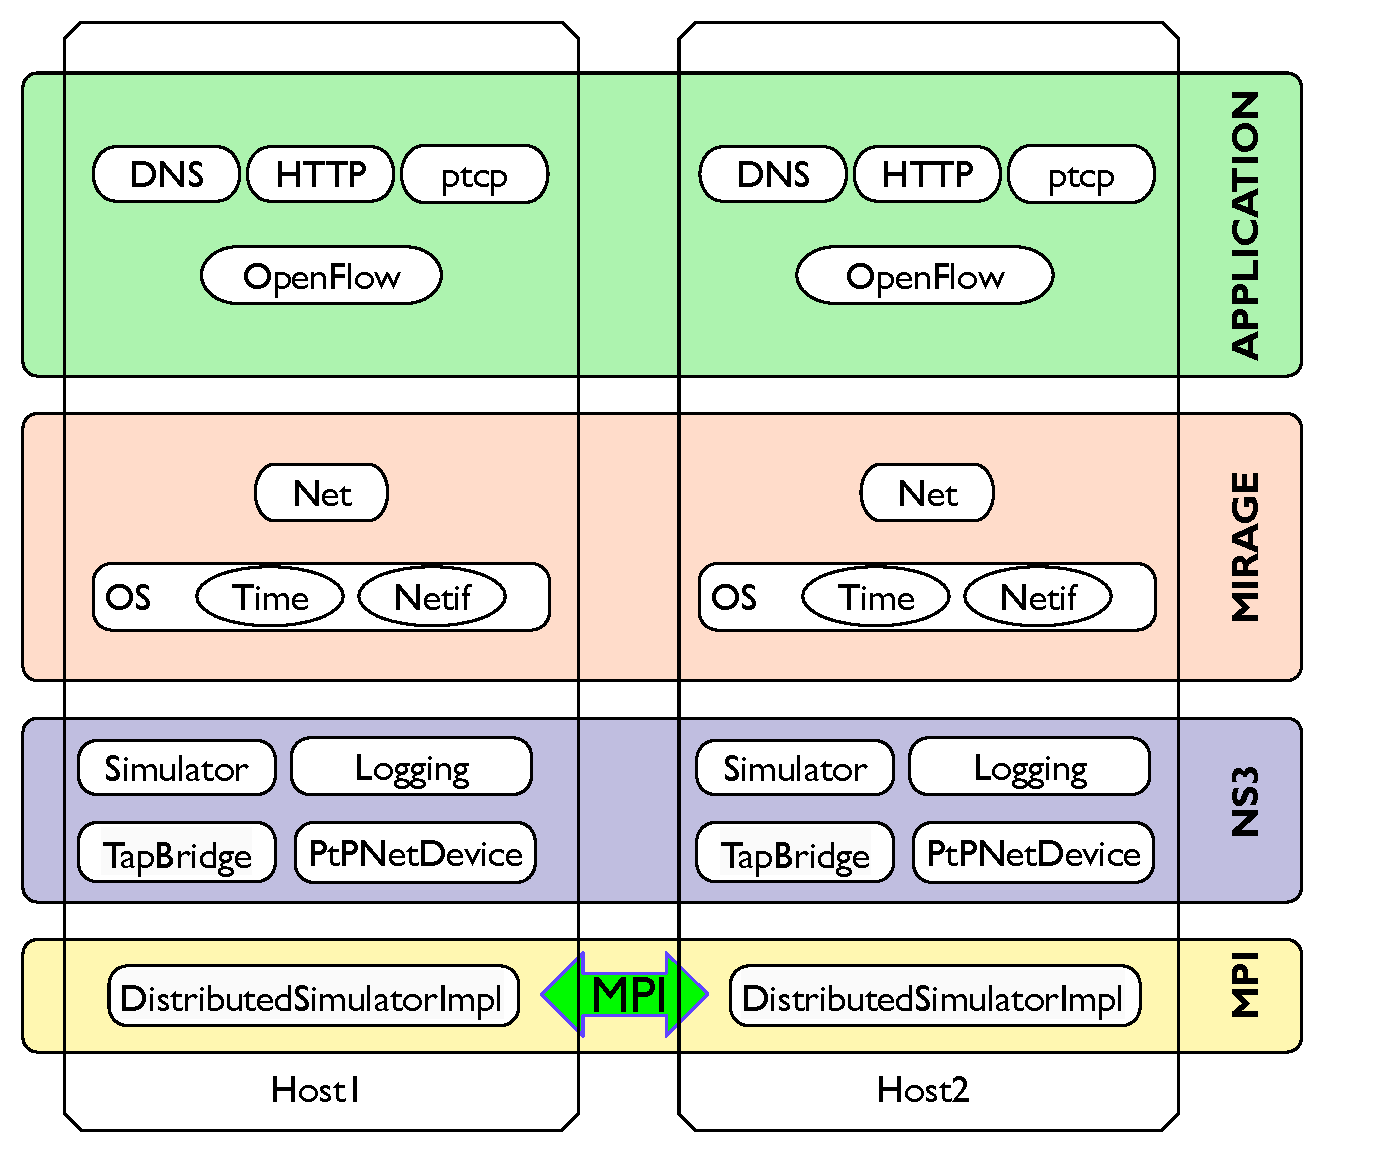
\includegraphics[width=0.45\textwidth]{sdnsim-arch-ns3}\label{fig:sdnsim-arch-ns3}}
\subfigure[Xen] {\includegraphics[width=0.45\textwidth]{sdnsim-arch-xen}\label{fig:sdnsim-arch-xen}}
\caption{\sdnsim host internal architecture: \ns{3}
  simulation~\ref{fig:sdnsim-arch-ns3} and xen real-time
  emulation~\ref{fig:sdnsim-arch-xen}.}
\label{fig:sdnsim-arch}
\end{figure}


\subsection{Xen backend}

An \sdnsim emulation host uses a simple PV Boot mechanism. At startup \sdnsim
initializes a VM with a single virtual CPU, loads the Xen event channel and
jumps to the main function of the OS module which runs the thread scheduling
loop.  \sdnsim uses the OCaml Lwt language extension, an event-driven
asynchronous programming library, to enable a multi-threading programming
abstraction.  Using the Lwt syntax, a developer can spawn new threads by
annotating closures as blocking. An Lwt thread is either executing code or idles
waiting for an IO event or a synchronisation primitive (e.g.~a semaphore) or a
timer timeout.  Lwt threads are cooperative and non-preemptive and the main
scheduling loop works as follow: Execute any resumable sleeping threads,
calculate the time left until the next timer event and poll for events from the
event channel until that time expires.  Timing integration with the Xen platform
is achieved through the Xen shared\_info struct, a structure containing CPU time
information which is shared between the Dum0 and the DumU VMs.  Network
integration is implemented using the Xen NetFront driver and the Xen event
channel.

\sdnsim uses the Xen Managment API~(XAPI)~\cite{xapi} to bootstrap emulations over
the XEN platform.  \sdnsim is able to create, start and stop VM instances and
configure network topologies.  Network topologies are implemented using  VM Virtual
Network Interface (VIF) bridging in the Dum0. A link between two hosts in an
experiment definition is translate to a layer-2 bridge which contains a VIF from
each VM\@.  XAPI also expose an interface to control link rate and propagation
delay for each VIF\@. In a Xen-based emulation of an \sdnsim experiment, the
emulation setup pipeline works as follows: host definitions are compiled in VM
images and equivalent VM definition are configured through XAPI, network
topology description is translated into equivalent bridge setup and, once all
configurations are completed, all VMs are booted.

\subsection{\ns{3} backend}

\ns{3}~\cite{Henderson2006} is a discrete-time packet-driven network simulation
framework. The core of the system consists of a discrete time simulation engine
and a set of \ns{3} libraries providing network
applications, routing protocols, data-link layer protocols and link emulations
models. \ns{3} is fundamentally an extensive refactor of the \ns{2} code-base
and provides a stable core of network functionality over which users can develop
custom simulation scenarios. 

The \ns{3} backend has a significant difference from the Xen backend; the
execution model is discrete and non-reentrant. \ns{3} applications can only
register their interest for specific time and network events, event handling is
atomic and the progress of the simulation is centrally controlled by the
simulation engine. In order to port the Lwt library to the \ns{3} simulation
engine, we transform thread blocking calls into equivalent \ns{3} events.  More
specifically, the Mirage OS clock abstraction is bridged with the \ns{3} simulation
clock and all sleep calls are scheduled as \ns{3} time events.  A thread is
resumed from a sleep call when the simulator executes the respective time event.
Network blocking calls are integrated with the network device abstraction of
\ns{3}.  The packet reading thread registers a packet handler on the network
device, while the packet writing thread checks the device queue occupancy and
blocks while the queue is full. Finally, in order to avoid scheduling deadlocks,
the OS schedules {\it idle} \/time events that resume any yielded threads. Using
these transformations we are able to provide a semantically accurate Lwt
integration with the \ns{3} engine.  Network links between hosts are simulated
using the {\it PointToPoint} \/link model. This model simulates a PPP link over a
lossless medium, a valid approximations for the full duplex non-shared medium of
current network datacenters.

Finally, in order to increase the scalability of the \sdnsim simulation backend,
we use a distributed version of the \ns{3} simulation engine. The simulation
engine spawns a different process for each host of the simulation and an
MPI-based synchronisation algorithm establishes conservative clock
synchronisation and distributed event execution~\cite{Pelkey:2011ua}. 

\section{\sdnsim evaluation} \label{sec:sdnsim-precision}

We evaluate performance and precision of the \sdnsim platform using small scale
micro-benchmarks that target the performance of the \of protocol library, as
well as, the scalability of the \ns{3} backend.  In~\cite{madhavapeddy2013},
there is an exhaustive analysis of the performance of the \mirage platform,
which we omit from this section. In the rest of this section we compare the
performance of our \mirage \of controller (Section~\ref{sec:of-controller-perf})
and \mirage \of switch (Section~\ref{sec:of-switch-perf}) with existing
equivalent software packages and evaluate the scalability of the \ns{3} backend
(Section~\ref{sec:sdnsim-ns3-perf}).
% \subsection{\of library performance} \label{sec:of-perf}

\subsection{\mirage Controller Emulation} \label{sec:of-controller-perf}

We benchmark our controller library's performance through a simple baseline
comparison against two existing \of controllers, NOX and Maestro.
NOX~\cite{nox} is one of the first and most mature open-source \of controllers;
in its original form it provides programmability through a set of C++ and Python
modules.  In our evaluation we compare against both the master branch and the
{\it destiny-fast} \/branch, an optimised version that sacrifices Python
integration for better performance.  Maestro~\cite{cai2011} is a Java-based
controller designed to provide service fairness between multiple \of control
channels.  We compare these controllers against our Xen-based \mirage \of
controller application.

Our benchmark setup uses the {\it Cbench}~\cite{cbench} measurement tool. Cbench
emulates multiple switches which simultaneously generates {\tt packet\_in}
messages.  The program measures the processing throughput of each controller.
It provides two modes of operation, both measured in terms of {\tt packet\_in}
requests processed per second: {\it latency}, where only a single {\tt
  packet\_in} message is allowed in flight from each switch; and {\it
  throughput}, where each emulated switch maintains a full 64\,kB buffer of
outgoing messages. The first measures the throughput of the controller
when serving connected switches fairly, while the second measures absolute
throughput when servicing requests from switches.
                                                                       
We emulate 16 switches concurrently connected to the controller, each serving
100 distinct MAC addresses. We run our experiments on a 16-core AMD server
running Debian Wheezy with 40\,GB of RAM and each controller configured to use a
single thread of execution. We restrict our analysis to the single-threaded case
as the Mirage execution environment, at time of testing, does not support
multi-threading. For each
controller we run the experiment for 120\,seconds and measure the per-second
rate of successful interactions. Table~\ref{tbl:controller} reports the average
and standard deviation of requests serviced per second.

Unsurprisingly, due to mature, highly optimised code, {\emph NOX fast} shows the
highest performance for both experiments. However, the controller exhibits
extreme short-term unfairness in the throughput test.  {\emph NOX} provides
greater fairness in the throughput test, at the cost of significantly reduced
performance. Maestro performs as well as NOX for throughput but significantly
worse for latency, probably due to the overheads of the Java VM\@.  Finally,
\mirage throughput is somewhat reduced from NOX fast but substantially better
than both NOX and Maestro. In addition, the \mirage controller achieves the best
product of performance and fairness among all tested controllers in the
throughput test.  Comparing latency, \mirage performs much better than Maestro
but suffer somewhat in comparison to NOX\@. From the comparison results, we
conclude that the \mirage controller performance is comparable to the
performance of existing controlling platforms and our emulation environment can
reproduce the performance of realistic \of deployment. 

\begin{table}
\newcommand\T{\rule{0pt}{2.6ex}}
\newcommand\B{\rule[-1.2ex]{0pt}{0pt}}
\centering
\begin{tabular} {l |r@{.}l r@{.}l|r@{.}l r@{.}l}
\hline
\T \multirow{2}{*}{Controller} 
   & \multicolumn{4}{c|}{Throughput (kreq/sec)}  
   & \multicolumn{4}{c}{Latency (kreq/sec)} \\
\B & \multicolumn{2}{c}{avg} & \multicolumn{2}{c|}{std.\ dev.} 
   & \multicolumn{2}{c}{avg} & \multicolumn{2}{c}{std.\ dev.} \\
\hline
\T NOX fast   & 122&6 & \quad{} 44&8 & 27&4 & \quad{} 1&4 \\
NOX           &  13&6 &  1&2 & 26&9 & 5&6 \\
Maestro       &  13&9 &  2&8 &  9&8 & 2&4 \\
\B Mirage Xen &  98&5 &  4&4 & 24&5 & 0&0 \\
\hline
\end{tabular}
\caption{\label{tbl:controller}OpenFlow controller performance.}
\end{table}

\subsection{\mirage Switch} \label{sec:of-switch-perf}

We benchmark our \mirage \of switch implementation through a baseline comparison
with the \ovs~(OVS)~\cite{openvswitch} kernel implementation.  We
develop, using the \oflops framework, a simple forwarding test and measure the
switching latency incurred by each implementation.  For this experiment we use
two virtual machines, one running the \oflops code, the other running the
\of switch configured with three interfaces bridged separately in dom0. One
interface provides a control channel for the switch, while the other two are
used as the switch's data channels. Using \oflops, we generate packets on one of
the data channels and receive traffic on the other, having bootstrapped appropriate
the switch flow table. We run the test for
30\,seconds, a sufficient measurement period to detect statistically significant
results. We use small packets (100\,bytes)\footnote{we use a packet size
  slightly larger that the minimum packet size because we append in the
  payload packet generation information~(e.g.~packet ID, packet generation
  timestamps).} and vary the data rate.

\begin{figure}
\centering
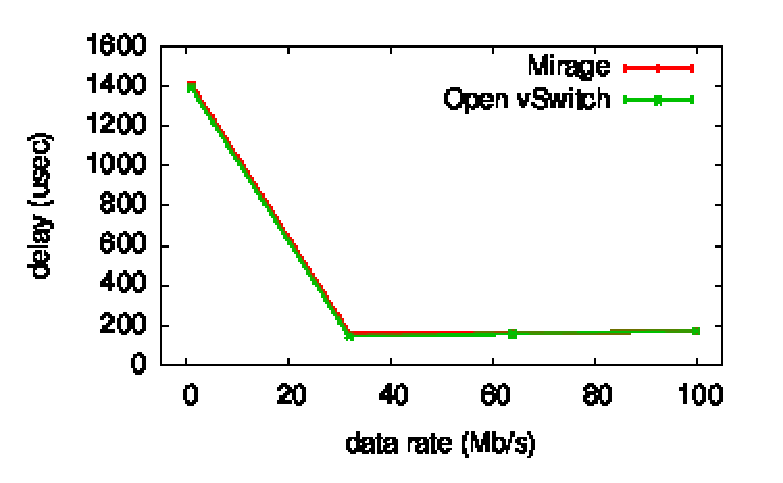
\includegraphics[width=\columnwidth]{switch-media-delay}
\caption{\label{fig:switch}Min/max/median delay switching 100\,byte packets
        when running the Mirage switch and \ovs kernel module as domU
        virtual machines.}
\end{figure}

Figure~\ref{fig:switch} plots as error boxes the min, median and max of the
median processing latency of ten test runs of the experiment. We can see that
the \mirage switch's forwarding performance is very close to that of the \ovs,
even mirroring the high per-packet processing latency with a probe rate of
1\,Mb/s; we believe this is due to a performance artefact of the underlying dom0
network stack. We omit packet loss, but can report that both implementations
suffer similar levels of packet loss.  From the comparison results of the
\mirage \of switch, we can conclude, that our \of switch can emulate accurately 
software
switch functionality. Nonetheless, the minimum latency of our switch emulation
(approximately 100 msec) is 2 order of magnitude higher than a hardware switch
(approximately 0.5-1 $\mu$sec). In order to bridge this latency gap, we propose
the introduction of a slowdown factor in the emulation.  A slowdown factor of
ten will reduce by ten times the time reported by the clock abstraction of the
\mirage platform and by ten the link rate allocated to each VIF\@. As a result,
the slowdown factor can provide a semantically correct slowdown to the time of
the experiment and use more efficiently the computational resources of the
server. 
% However, the \mirage switch has a memory footprint of just 32\,MB compared with
% the \ovs virtual machine requirement of at least 128\,MB. We aim
% to improve integration of the Mirage switch functionality
% with the Xen network stack to achieve lower switching latency. Nonetheless,  

\subsection{\ns{3} performance} \label{sec:sdnsim-ns3-perf}

\begin{figure}[ht]
\subfigure[centralised topology]{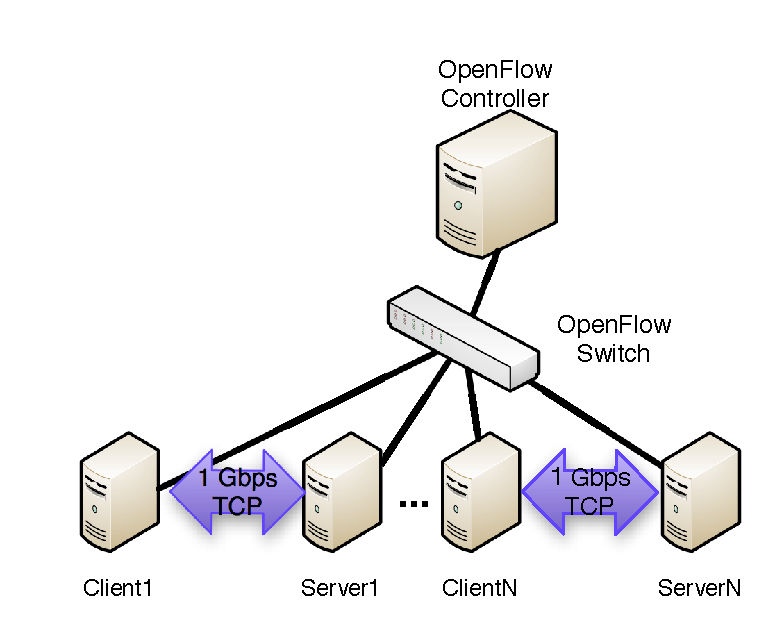
\includegraphics[width=0.45\textwidth]{sdnsim-topology-single}\label{fig:sdnsim-ns3-simulation-single}}
\subfigure[distributed topology] {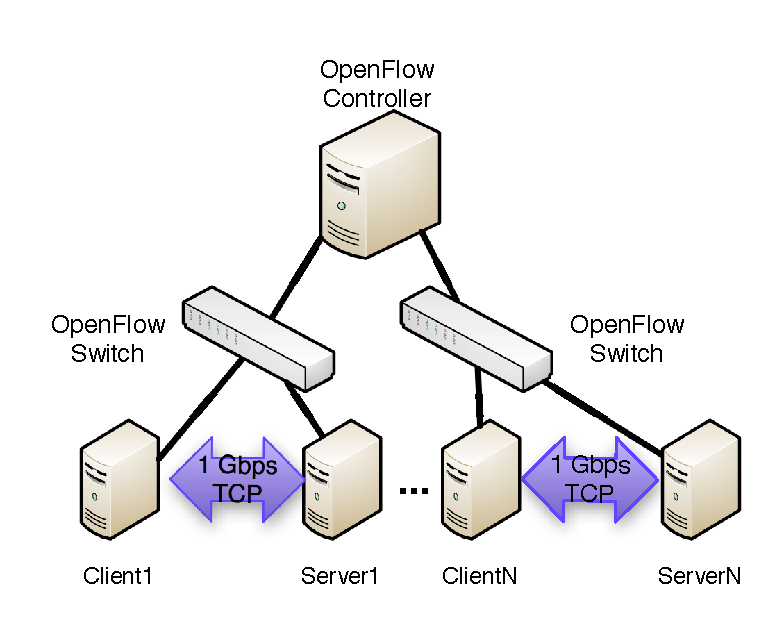
\includegraphics[width=0.45\textwidth]{sdnsim-topology-double}\label{fig:sdnsim-ns3-simulation-double}}
\caption{Network topology to test the scalability of \ns{3}-based simulation. We
simulate two topologies: a centralised
topology~(Figure~\ref{fig:sdnsim-ns3-simulation-single}) and a distributed
topology~(Figure~\ref{fig:sdnsim-ns3-simulation-double})}
\label{fig:sdnsim-ns3-simulation}
\end{figure}

\begin{table}
\begin{center}
\begin{tabular}{|l|c|c|c|c|c|c|} \hline
&\multicolumn{3}{|c|}{Centralised topology} & \multicolumn{3}{|c|}{Distributed
  topology} \\
\cline{2-7}
Number of hosts & 4 & 8 & 12 & 4 & 8 & 12 \\
\hline 
Wall-clock delay (in min) & 13 & 35 & 75 & 8 & 25 & 42 \\
\hline
Slowdown factor & 26 & 70 & 150 & 16 & 50 & 84 \\
\hline 
\end{tabular}
\end{center}
\caption{Wall-clock delay to run a 30 seconds simulation time of the topology
  presented in Figure~\ref{fig:sdnsim-ns3-simulation}, for variable number of network hosts. 
  \sdnsim simulation of a network experiment using the \ns{3} backend
  scales linearly as the traffic is localised. }
\label{tbl:sdnsim-ns3-simulation-results}
\end{table}

In order to test the scalability of \sdnsim simulation we implement a
simple network experiment, depicted in Figure~\ref{fig:sdnsim-ns3-simulation}.
The topology consists of a number of switches and host pairs,
connected through 1 Gbps links.  Each pair of hosts generates steady
state TCP traffic at line rate.  We use two variations of the topology: A {\it
  centralised topology} \/with all the pairs of hosts connected to a single
switch~(Figure~\ref{fig:sdnsim-ns3-simulation-single}), and a {\it distributed
  topology}, with pairs of hosts distributed between two switches and traffic
remaining local to the switch~(Figure~\ref{fig:sdnsim-ns3-simulation-double}).
Each switch is connected to an \of controller that implements a learning switch.
The experiment executes 30 seconds of simulation time on a 24-core AMD server
with 128 GB of RAM. 

In Table~\ref{tbl:sdnsim-ns3-simulation-results}, we present the wall-clock
execution time and the slowdown factor of each simulation.  From the results we
note that the real time to execute a simulation in \sdnsim depends on the number
of network events; as we increase the number of host and, consequently, the
number of packets, the execution time increases.  Additional, from the
comparison between the centralised and distributed topology, we note that the
performance of the simulation improves when network events are localized, as the
simulation can be parallelized. In the distributed topology, network events are
distributed between the two switch and they execute independently, achieving
near-linear scaling. These scaling properties of the \sdnsim simulation
implementation provide a scalable experimentation framework for datacenter
traffic models and designs~\cite{Kandula09}. 

% The results show
% that the platform can scale close to linear when the hosts of the simulation
% create small autonomous partition.  In the centralised topology, the \of switch
% becomes a bottleneck of the simulation, since it has to process sequentially all
% network events. For the distributed topology, the distributed nature of the
% event engine permits parallelization of the event processing between the two
% switches, thus reducing the experiment running time. Although the simulation
% scenario 

\section{hierarchical control distribution in Software-defined network} 
\label{sec:rdsf-eval}
%%%%%%%%%%%%%%%%%%%%%%%%%%%%%%

% \section{\sdnsim conclusions} 

\begin{table}
\begin{center}
\begin{tabular}{|c| l |} \hline
  Parameter & value \\ \hline
  packet\_in processing delay & 10 msec \\ \hline
  flow\_mod insertion delay & 1,2 msec \\ \hline
  link capacity & 1 Gbps \\ \hline
  Request arrival rate & 1500 retrievals/sec \\ \hline
  link propagation delay & 0.5 $\mu$sec \\ \hline
  switch processing delay & 100 $\mu$sec \\ \hline
\end{tabular}
\end{center}
\label{tbl:sdnsim_experiment_parameters}
\caption{control hierarchy simulation parameters}
\end{table}

The \of abstraction provides an excellent mechanism to centralise control in a
network and avoid the performance overhead of existing distributed control plane
protocols. Using \of, allows to offload the control plane of all switches of a
network to a single centralised network controller which has full knowledge of
the network state and construct an optimal routing policy.  Nonetheless, as the
network size increases, the centralisation strategy will face significant
problem to scale centrally the control plane requirements.  Large networks
require a mechanism to distribute the control computation over multiple
tightly-coupled controllers. In order to address this requirement we use \sdnsim
to test a hierarchical control system. In our control architecture, we propose
the introduction of a hierarchy of controllers which control a subset of the
switch devices and a subspace of the \of tuple space. In order to enable control
distribution, as well as, responsive control, each node of the hierarchy run a
flowvisor instance to multiplex switch control channels. The flowvisor is
configurated to delegate control to a local controller, while also propagating
control events to upper layers of the hierarchy in order to build higher level
controllers which construct global view of the network and enforce higher
priority control policies. In order to understand the impact of this control
hierarchy, we use \sdnsim, to simulate the control architecture and evaluate the
impact of multi-level control schemes on the performance of the data plane. 

In our experiment we use a FatTree~\cite{Al-Fares08} network topology with 4
pods and simulate a small-scale datacenter. For data plane traffic we use a
simple client-server architecture to replicate the functionality of data
retrievals in Map-Reduced platforms. In the network we assign the machines
hosted in the first three pods to function as data requesters and the machines
hosted in the forth pod to function as data providers. Each data request
consists of a small 10 bytes packet from the requester, to define the number of
bytes which will be send subsequently by the data provider. The traffic size of
the request is selected uniformly at random between the values 4KB, 8KB and
32KB.  The request arrival rate follows a Poisson model, while the destination
is choose uniformly at random between the servers of the forth pod. In addition,
each client keeps a persistent long-lived background TCP connection. Using this
simple model we can experiment with traffic models similar to a datacenter
network. In the control of the network we simulate the control logic of the
FatTree design: every 1 second the network control receives flow-level
statistics from the switch and reassign network flows in order to reduce link
utilisation and spread the load between redundant. In order to study the effects
of our architectural approach, we variate the number of FlowVisor instances
which process \of traffic before reaching the local controller of the switch and
study the impact of the proximity of the controller on data plane performance,
by measuring the completion time of each network flow. Further parameters of the
simulation are described in Table~\ref{tbl:sdnsim_experiment_parameters}.


\section{Summary} \label{sec:modeling:summary}


% \section{\oflops Conclusions}\label{sec:conclusion}
%%%%%%%%%%%%%%%%%%%%%%%%%%%%%%
% \todo{Add some notes on \sdnsim}

This chapter discusses the scalability capabilities of the predominant SDN
implementation, the \of protocol.  We presented, \oflops, a tool that tests the
capabilities and performance of OpenFlow-enabled software and hardware switches.
\oflops combines advanced hardware instrumentation, for accuracy and
performance, and provides an extensible software framework. We use \oflops to
evaluate five different \of switch implementations, in terms of OpenFlow
protocol support as well as performance.  In our performance evaluation, we
benchmark the packet processing, traffic interception and injection, flow table
modification and traffic statistics export functionalities of the switches.  We
identify considerable variation among the tested \of implementations.  We take
advantage of the ability of \oflops for data plane measurements to quantify
accurately how fast switches process and apply \of commands.  For example, we
found that the \texttt{barrier} reply message is not correctly implemented,
making it difficult to predict when flow operations will be seen by the data
plane.  Finally, we found that the monitoring capabilities of existing hardware
switches have limitations in their ability to sustain high rates of requests.
Further, at high rates, monitoring operations impact other OpenFlow commands.

In addition, in this chapter we present the \sdnsim platform, an experimentation
framework for large-scale high-precision experimentation with control plane
architectures. \sdnsim reuses the \mirage systems abstraction layer to enable
developer to program the functionality of their network. An \sdnsim experiment
definition can seamlessly translate at compile into a simulation over the \ns{3}
simulation platform, or a high precision emulation over the Xen virtualization
framework. We conduct a number of micro-benchmarks and evaluate that the
software provide emulation performance comparable to software \of controller and
switching platforms, while \sdnsim simulation provide good scaling properties.
Furthermore, using \sdnsim we investigate the impact of hierarchical distributed
control architectures on the performance of the data plane of the network.  In
the next chapter, we explore applications of the SDN paradigm to scale network
management. 

%We also readily acknowledge this paper as a snapshot of work in
%progress; every set of results poses new questions but also the role
%of \oflops can evolve as new OpenFlow instantiations are introduced and
%existing ones refined; considerable opportunity exists for future
%work.

% LocalWords:  Oflops OpenFlow

%%% Local Variables: 
%%% mode: latex
%%% TeX-master: "../thesis"
%%% End: 
